%\part{Contas Sem Identidade}
\chapter{Contas Sem Identidade}
\label{ch:capitulo7}

Até agora, construímos um livro-razão distribuído sem autoridade central, um sistema de loteria para selecionar quem escreve, um sistema para recompensar bons mineradores e punir os que se comportam mal, uma forma de ajustar a dificuldade de mineração para garantir um cronograma de cunhagem consistente e reduzir conflitos, e um sistema para verificar a validade da cadeia, examinando a prova cumulativa de trabalho e o histórico de transações.

Agora vamos lidar com a identidade. 
Em um sistema bancário tradicional, você envia dinheiro identificando-se ao banco, seja por meio da apresentação de um código ou PIN pessoal ou da apresentação do nome de usuário e senha, no aplicativo. 
O banco garante que duas pessoas não compartilhem uma só identidade.

Já que agora não temos uma entidade central para rastrear os indivíduos, como podemos abrir contas em nosso novo sistema financeiro baseado em Bitcoin?
Como podemos encaminhar para objetivo de Satoshi de remover identidade de transações financeiras, afim de evitar furto de identidades e entidades centrais.%adicionado e furto de identidade
Como podemos garantir que, quando \TraducaoNomeA anunciar que deseja pagar \TraducaoNomeB, seja realmente ela e, tenha a autoridade de enviar esses fundos?

\section*{Gerando uma “Conta Bitcoin”}
%\paragraph{}

Já que não podemos contar com um intermediário central como um banco para manter um registro de todas as contas.
%e como as pessoas podem entrar e sair quando quiserem, sem permissão, como podemos gerenciar suas contas?        removido
E se permitirmos que todos registrem seu próprio nome de usuário e senha?
Um banco normalmente verifica se um nome de usuário ainda não está em uso, mas isso não é possível neste caso, já que não temos um ator central distribuindo identidades. 
Portanto, precisamos de algo maior, mais forte e mais exclusivo do que um nome de usuário e uma senha. 
Esta técnica deve ser semelhante aos capítulos anteriores. Mais uma vez, precisamos de um número aleatório gigante.

Assim como possibilitamos que todos comprassem bilhetes de loteria gerando grandes números aleatórios, podemos usar o mesmo truque para gerar contas. Para criar uma “Conta Bitcoin”, também conhecida como endereço, primeiro geraremos um par de números de 256 bits matematicamente vinculados, conhecido como \textit{par de chaves pública/privada}. Novamente, \(2^{256}\) é tão grande quanto o número de átomos no universo, então duas pessoas gerando acidentalmente o mesmo par de chaves é quase impossível.
Daremos o nosso endereço a qualquer pessoa que queira nos enviar moedas. Usaremos a chave privada para gastar as moedas.%adicionando
É assim que elas funcionam.%adicionado

Criptografia é um método para pegar dados e obscurecer eles, de tal maneira que só quem tem acesso a chave consegue ler a mensagem original através de descriptografar.
Como crianças alguns de nos brincávamos com brinquedos codificadores e decodificadores para converter uma mensagem em lero-lero e retornar ela a uma mensagem normal depois.
Esse tipo de criptografia é chamada de simétrica pois usa apenas uma chave. 
O par de chaves tem algumas propriedades interessantes. Você pode usar qualquer uma das chaves para criptografar uma mensagem e a outra para descriptografá-la.

Você está convidado a compartilhar sua chave pública com o mundo inteiro. Saber essa chave não permite que eles tenham acesso à sua chave privada.
Pessoas que queiram te enviar uma mensagem podem criptografar elas com tua chave publica.
Porque apenas você tem a chave privada, você é o único que consegue descriptografar a mensagem.

Vamos dar uma olhada qual o processo que \TraducaoNomeA faz para enviar as moedas para \TraducaoNomeB.
Para receber uma transação, \TraducaoNomeB gera um par de chaves privadas/públicas e mantém sua chave privada em segredo. 
Ele produz um \textit{endereço}, um grande número com base no hash da sua chave pública. 
\TraducaoNomeB, então, compartilha esse número de endereço com \TraducaoNomeA para que ela possa enviar moedas para ele.

você pode pensar que endereços são caixas postais. 
Invés de cartas, \TraducaoNomeA pode depositar moedas nesse caixa postal. 
Mas apenas \TraducaoNomeB possui a chave privada que vai abrir o caixa postal, liberando ele à gastar essas moedas.

Quando movimentas dinheiro dentro de um banco, você fornece a eles um usuário e senha.
Quando escreves um cheque, você assina seu nome para autenticar que você escreveu o cheque.
Quando movimentas bitcoins, você fornece uma prova que es o dono da chave para o endereço que detêm as moedas.

\TraducaoNomeA agora precisa informar à rede que está enviando moedas para o endereço público de \TraducaoNomeB à partir de seu próprio endereço público. Como ela prova que está autorizada a gastar naquele endereço público? Ela faz isso fornecendo prova de que possui a chave privada desse endereço, mas sem realmente revelar sua chave privada.

Essa prova de propriedade é chamada de \textit{assinatura digital}. Ana constrói uma transação, que essencialmente é apenas um pedaço de dados que parece algo como:

\begin{quote}
    “o endereço 12345 que contem 2.5 bitcoins, está enviando 2 bitcoins para o endereço 56789 e 0.5 bitcoins de volta ao endereço 12345”, 
\end{quote}

Exceto que os números do endereço são, na verdade, números gigantes de 160-bits. Ela então faz o hash de sua transação e criptografa o hash com sua chave privada, criando uma \textit{assinatura digital}.

Quando ela publica sua transação na rede, ela revela sua chave pública (de onde ela está enviando). Uma vez que todos possuem a chave pública, todos podem facilmente descriptografar a assinatura digital. 
\TraducaoNomeA anuncia o seguinte:

%Mas eles só seriam capazes de descriptografar se fosse, de fato, criptografado com a chave privada correspondente que apenas Ana conhece.

\begin{itemize}
    \item  estou enviando moedas do endereço 12345.
    \item Aqui esta a chave publica do endereço 12345, e vocês podem de fato ver que é a chave publica pelo hashando a chave publica e vendo que chegas no endereço.
    \item Aqui esta a assinatura digital que eu criptografei com a chave privada correspondendo a esse endereço. você pode usar a chave publica para descriptografar ele e verificar que é idêntica a transação que estou enviando.
\end{itemize}

\begin{figure}
    \centering
    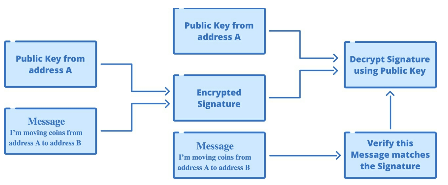
\includegraphics[width = 10cm]{imagens/capitulo7/Transação.png}
    \caption*{\textit{\small A transação que movimenta as moedas esta criptografada usando uma chave privada para criar um assinatura digital. Ela é descriptografada usando uma chave publica, que todos conhecem.}}
\end{figure}

Visto que agora todos tem a chave publica da \TraducaoNomeA, eles conseguem facilmente descriptografar a assinatura digital.
Pela virtude de ser capaz de descriptografar corretamente a assinatura utilizando a chave publica permite que todos saibam que \TraducaoNomeA tem a chave privada para aquele endereço.
Caso não tivesse, a descriptografia teria falhado, pois a chave publica pode apenas descriptografar mensagens criptografada pela chave privada.
É importante ressaltar que não foi revelado sua chave privada, eles tem apenas a prova que ela foi capaz de utilizar a chave privada criptografando a assinatura.

%Quando você move dinheiro em um banco, você fornece a eles seu nome de usuário e senha. Quando você passa cheques, assina seu nome para autenticar que é você quem está escrevendo o cheque. Ao mover o bitcoin, você prova que possui a chave do endereço que contém o bitcoin.

Ao contrário de uma assinatura em um cheque ou de sua senha de banco, sua assinatura digital é específica para os dados de transação exclusivos que você está assinando. Portanto, não pode ser roubada e reutilizada em uma transação diferente. Cada transação recebe uma assinatura diferente, mesmo que seja baseada na mesma chave privada, visto que qualquer informação modificada muda o hash da assinatura.

%\newpage
\section*{Você consegue adivinhar uma chave privada?}
%\paragraph{}

Vamos descobrir as chances de adivinhar uma chave privada, o que lhe daria a capacidade de mover as moedas no endereço público correspondente. Lembre-se de que uma chave é composta por 256 bits. Cada bit possui apenas dois valores (um ou zero). Isso significa que você pode visualizar cada bit como um cara ou coroa.

Se tivéssemos uma chave privada de 1 bit, seria como jogar uma moeda. Cara ou coroa, um ou zero? Você tem uma chance em duas de acertar.

Revisão rápida de probabilidade básica: A probabilidade de ocorrência de vários eventos é calculada multiplicando-se a probabilidade individual de cada evento. Se um lançamento de moeda tem 1/2 chance de dar cara, então a chance de dois lançamentos de moeda consecutivos dar cara é $1/2 x 1/2 = 1/4$ ou 1 em 4.

%Se tivéssemos 2 bits, seriam dois lançamentos de moeda consecutivos. $(2^2) = 4$, então você tem uma chance em 4.

Se você adivinhasse o resultado de 8 lançamentos consecutivos de moeda, seria $(2^8)$, ou uma chance em 256.

Uma placa de carro americana tem 6 letras e números. Existem 26 letras e 10 números, portanto, um total de 36 caracteres. Como há seis deles, o número de placas de carros possíveis $= (36^6)$, então suas chances de adivinhar a minha são de uma em 2.176.782.336 (uma em dois bilhões).\footnote{A inspiração para esta seção veio de uma excelente postagem no Medium que detalha as probabilidades de uma variedade de eventos. Recomendo a leitura da postagem completa para contexto: \url{https://medium.com/breathe-publication/a-dance-with-infinity-980bd8e9a781}}.

Um cartão de crédito tem dezesseis dígitos. Cada dígito pode ter 10 valores, e há 16 deles, então suas chances de adivinhar meu cartão de crédito são de uma em $(10^{16})$, que é uma em 10.000.000.000.000.000.000 ou aproximadamente uma em dez quintilhões.

Existem cerca de $(10^{50})$ átomos na Terra. Se estou pensando em um ao acaso, suas chances de adivinhar exatamente qual átomo, é de:

%\begin{samepage}
\begin{quote}{Um em 1.000.000.000.000.000.000.000.000.000.000.\newline
000.000.000.000.000.000.000.}\end{quote}
%\end{samepage}

Uma chave privada tem 256 bits, que é \(2^{256}\) ou cerca de \(10^{77}\). Na verdade, está mais perto em magnitude de adivinhar um átomo específico de todo o universo ou de ganhar na Mega Sena 9 vezes seguidas usando apenas 6 números:

%\begin{samepage}
\begin{quote}{Uma chance em 115.792.089.237.316.195.423.570.985.\newline 008.687.907.853.269.984.665.640.564.039.457.584.007.\newline
913.129.639.936}\end{quote}
%\end{samepage}

Mas e se você tivesse um computador superpoderoso para fazer as suposições? Não posso fazer mais justiça a este assunto do que a este post\footnote{A postagem completa do Reddit que descreve como adivinhar uma chave de 256 bits está disponível aqui: \url{https://bit.ly/2Dbw9Qd}} do Reddit, que recomendo a leitura na íntegra. Embora seja técnico, o parágrafo final dá uma boa ideia do que seria necessário para listar todas as chaves de 256 bits possíveis:

\begin{quotation}\begin{samepage}
\enquote{Então, se você pudesse usar o planeta inteiro como um disco rígido, armazenando 1 byte por átomo, usando estrelas como combustível e percorrendo 1 trilhão de chaves por segundo, você precisaria de 37 octilhões de Terras para armazená-lo e 237 bilhões de sóis para alimentar o dispositivo capaz de fazer isso, o que levaria 3,6717 octodecilhões de anos.}
\begin{flushright} -- U/PSBLAKE EM R/BITCOIN
\end{flushright}\end{samepage}\end{quotation}

Basicamente, é impossível adivinhar a chave privada de alguém. Não apenas isso, mas o número de endereços de Bitcoin é tão grande que as melhores práticas realmente exigem a geração de um novo endereço para cada transação que você fizer. Então, em vez de ter uma conta bancária, você pode ter milhares ou até milhões de contas Bitcoin, uma para cada transação que já recebeu.

Pode ser desconcertante que sua conta Bitcoin seja protegida apenas por acaso, mas espero que a ilustração acima dê a você uma ideia de que isso é muito mais seguro do que a senha de sua conta bancária, armazenada em um servidor centralizado, disponível para hackers.

\section*{Rastreamento de saldos}
%\paragraph{}

É hora de corrigir uma última mentira inofensiva que já dissemos em capítulos anteriores. Na verdade, não há saldos mantidos no livro-razão. O Bitcoin usa um modelo chamado UTXO: Unspent Transaction Outputs.
A UTXO é simplesmente a palavra para uma saída de transação - uma moeda produzida por uma transação anterior, incluindo uma \textit{transação do tipo coinbase} de recompensa em bloco - que ainda não foi gasta em outro endereço.

Diferente de moedas metálicas que podem vir com uma determinada denominação, como por exemplo centavos, dezenas de centavos, 25 centavos, bitcoins são divisíveis em ate 100,000,000 unidades chamados de satoshis. 
Então dependendo do valor que recebeste nos seus endereços, talvez você precise combinar moedas de múltiplos endereços para gerar um UTXO maior, ou separar um UTXO para tornar ele menor. 
A ideia do UTXO é que cada transação é um conjunto de entradas que são consumidas para produzir novas saídas.
Pense nisso como enviar um monte de moedas para uma máquina que derrete e cunha novas moedas de qualquer valor que quisermos.
Carteira, que discutiremos mais tarde nesse capitulo, geralmente administram isso por trás das cenas, para que você precise apenas especificar a quantidade que deseja enviar.


Digamos que \TraducaoNomeA tenha um endereço que contém 1 bitcoin. Ela deseja enviar $0,3$ bitcoins para \TraducaoNomeB. Ela gera uma transação que mostra seu endereço com 1 bitcoin com o seu UTXO como entrada e duas saídas: um novo endereço bitcoin UTXO que vale $0,3$ como saída para o endereço do \TraducaoNomeB e um novo UTXO que vale 0,7 como saída para seu próprio endereço como troco.
O troco pode ir para o endereço de envio original ou, para melhor privacidade, ela pode enviá-la para um novo endereço que foi gerado instantaneamente.

Já que não há nenhuma maneira de dizer quem controla qual endereço na blockchain. 
Para isso, você precisa saber as chaves privadas correspondentes e vinculá-las às identidades do mundo real. 
O modelo UTXO incentiva um mecanismo de privacidade muito bom, permitindo a criação de novos endereços sempre que as moedas são movidas.
Então uma pessoa pode ter centenas ou milhares de endereços se eles enviam ou recebem moedas com frequência
Softwares de carteira fazem a gestão de tudo isso para a gente, evitando que precisamos nos preocupar com os detalhes.

Assim, para verificar o “saldo” de um determinado endereço, na verdade temos que somar todos os UTXOs que possuem este endereço como saída. 
O conjunto total de UTXOs atuais no Bitcoin aumenta quando as pessoas enviam de um endereço para vários e diminui quando as pessoas realizam transações de “consolidação” em que moedas de vários endereços são gastas em um endereço.

O modelo UTXO permite a validação fácil e eficiente de gastos duplos, uma vez que qualquer UTXO em particular só pode ser gasto uma vez. Não precisamos saber todo o histórico de gastos de uma conta específica.

Também podemos criar e destruir qualquer número de UTXOs de uma vez, criando transações complexas que misturam diferentes entradas e saídas.
Isso permite a ideia de “mistura de moedas”\footnote{\url{https://en.bitcoin.it/wiki/CoinJoin}}, em que várias partes participam de uma única transação de Bitcoin que mistura qualquer número de entradas para produzir qualquer número de saídas, obscurecendo assim o histórico dos UTXOs.
A popularidade de tais técnicas esta aumentando e é importante para privacidade e fungibilidade, que é um termo que dita que qualquer um bitcoin é equivalente a outro bitcoin.
Dessa maneira se alguns bitcoins caírem nas mãos de uma entidade desagradável, as moedas não são marcadas por toda a eternidade só porque foram utilizadas para algum ato nefasto.

%Ele também permite que as pessoas consolidem moedas de vários endereços para um ou espalhem-nas entre vários endereços para melhorar a segurança e a privacidade.
%\newpage

\section*{Carteiras}
%\paragraph{}

Como gerar uma conta nada mais é do que gerar um número aleatório de 256 bits para ser sua chave privada, e podemos criar milhares ou milhões de contas, precisamos de um mecanismo para rastreá-las. No Bitcoin, a palavra \textit{carteira} é usada para se referir a qualquer tipo de dispositivo que rastreia suas chaves. Pode ser tão simples como um pedaço de papel ou tão complexo como uma peça de hardware.

O software original do Bitcoin publicado por Satoshi veio com uma carteira de software. 
Essa carteira geraria seu par de chave pública/privada, geraria endereços e selecionaria UTXOs para você possa enviar bitcoins em qualquer valor.% (lembre-se novamente de que a chave pública é usada para criar seu endereço Bitcoin e sua chave privada permite que você assine transações para gastar moedas desse endereço).%revisar esse

Ao contrário da carteira do seu banco, que normalmente tem a forma de um único aplicativo móvel ou internet banking, o Bitcoin é um sistema completamente aberto. Portanto, existem centenas de carteiras, a maioria das quais é gratuita, sendo muitas delas também de código aberto, bem como meia dúzia de implementações de carteiras de hardware, com outras sendo produzidas. Qualquer pessoa com conhecimento de programação de computadores pode construir sua própria carteira ou ler o código de uma carteira de código aberto para garantir que nada de suspeito esteja acontecendo. 

Este é outro lugar no Bitcoin onde a inovação sem permissão está acontecendo em um ritmo rápido, ao contrário do aplicativo móvel do seu banco.%nao possui

Visto que sua chave privada é a única coisa de que você precisa para gastar suas moedas, você deve guardá-la bem. Se alguém roubar seu cartão de crédito, você pode ligar para a empresa e registrar uma reclamação de fraude e tentar obter seu dinheiro de volta. No Bitcoin, não há intermediário. Se alguém tem sua chave privada, eles controlam suas moedas e não há ninguém que você possa ligar.

As chaves privadas também são altamente suscetíveis a perdas. Se você armazenar sua carteira no computador e ele for roubado ou pegar fogo, você tem um problema. Se você seguir as práticas recomendadas do Bitcoin para gerar um novo endereço toda vez que receber um pagamento, armazenar e fazer backup com segurança dessas chaves privadas se tornará algo muito custoso.

Com o tempo, o ecossistema Bitcoin desenvolveu uma série de soluções para esse problema. Em 2012, o BIP32 (Bitcoin Improvement Proposals ou Proposta de Melhoria do Bitcoin, um mecanismo para as pessoas espalharem ideias sobre como melhorar o Bitcoin) foi proposta para criar Carteiras Determinísticas Hierárquicas. A ideia por trás disso é que usando apenas um único número aleatório (seed), podemos gerar uma cadeia inteira de pares de chaves públicas/privadas: endereços de Bitcoin e chaves de assinatura para eles.

Hoje em dia, se você usar qualquer um dos softwares comumente disponíveis ou carteiras de hardware, eles gerarão automaticamente novas chaves para você para cada transação e permitirão que você faça backup de apenas uma única seed.

Em 2013, o BIP39 veio para tornar o backup de chaves ainda mais fácil. Em vez de usar um número completamente aleatório, as chaves seriam geradas a partir de um conjunto aleatório de palavras que seriam legíveis por seres humanos. Aqui está um exemplo de seed:

\begin{samepage}
\begin{quote}{witch collapse practice feed shame open despair creek road again ice least}\end{quote}
\end{samepage}

Com esse método, o backup das chaves se tornou muito fácil: você pode escrever a seed em um pedaço de papel e colocá-la em um cofre. Você pode até memorizar a frase e sair de um regime econômico decadente como a Venezuela, sem que ninguém saiba que você está carregando sua riqueza na cabeça.

Além disso, um endereço Bitcoin pode exigir mais de uma chave privada para ser acessado. Endereços multisignature ou \textit{multisig} podem empregar uma grande variedade de esquemas de segurança. Por exemplo, duas pessoas podem compartilhar uma conta usando multisig 1 de 2, onde qualquer uma das partes pode assinar as transações e gastar as moedas.

Um multisig 2 de 2, que exige que ambas as partes forneçam as chaves privadas para gastar, impedindo de qualquer uma pessoas possa controlar as moedas, utilizada por exemplo entre parceiros comerciais.



Você pode fazer um sistema de depósito simples usando um multisig 2 de 3. O comprador obtém uma chave, o vendedor obtém outra chave e uma terceira chave é dada a um verificador. Se o comprador e o vendedor concordarem, eles podem desbloquear os fundos sem a necessidade do verificador.
Em caso de litígio, o verificador pode agir em conjunto com uma das partes para desbloquear os fundos.

Você pode usar um esquema multisig 3 de 5 para se proteger contra a perda de chaves, permitindo-se perder até 2 das 5 chaves e ainda ser capaz de desbloquear a conta. Você pode armazenar duas das chaves em lugares diferentes, duas com amigos de confiança diferentes que não se conhecem e uma com um serviço de custódia especializado como o BitGo que assina suas transações, tornando seu Bitcoin muito difícil de ser roubado enquanto se protege das perdas das chaves.

Você pode ir ainda mais longe e criar endereços que são desbloqueados por condições bastante complexas utilizando construtos de programação como frases condicionais por exemplo "se isso então aquilo" (\textit{if this then that}).
Você pode, por exemplo, fazer um endereço de bitcoin do qual você não pode gastar por 10 anos, não importa o quanto alguém queira forçá-lo a mudá-lo.

Mais e mais soluções semi custodiais estão surgindo de empresas como Casa ou Unchained capital, que te ajudam a armazenar suas chaves de uma maneira segura. Diferente de um banco que pode congelar sua conta, essas soluço es parcialmente custodiais atuam como um backup ou coassinante de confiança, mas não podem eles mesmos tirar os fundos sem suas chaves.
Carteira estão constantemente evoluindo porque não requer a permissão de ninguém para fazer isso, diferente do aplicativo do seu banco. 
Por conta disso vemos novas entidade surgindo e mais inovação o tempo todo.

Isso é profundo e transforma o mundo. Nunca antes foi possível transportar seus bens de uma forma completamente segura contra apreensão ou roubo.